\setauthor{Moritz Eder}

Die heutige Welt und der Alltag werden immer schneller und komplexer,
was für viele Menschen einen Stress verursacht.

\begin{itemize}
    \item Gesundheit ist ein wichtiger Faktor.
    \item Oft fehlt die Möglichkeit sich zu entspannen.
    \item Viele Menschen leiden darunter.
    \item Die Betroffenen verlieren den Mut sich Hilfe zu holen.
\end{itemize}

Stress bewirkt bei Menschen oft nicht nur enormen Leistungsdruck, sondern er kann auch zu gesundheitlichen
Folgen führen. Mögliche Folgen von hohem Stress oder hohem Leistungsdruck könnten sein:

\begin{itemize}
    \item Zeichen von Nervosität
    \item Verspannungen, die zu Kopf-, Genick- und Rückenschmerzen führen können
    \item Vergesslichkeit
    \item Depression
    \item psychische Störungen
\end{itemize}

Anhaltender Stress kann sogar Herz/Kreislauf- und Nierenerkrankungen, Stoffwechselstörungen, Allergien oder
Entzündungskrankheiten hervorrufen. \cite{stress} Daher benötigen gestresste Menschen eine Möglichkeit sich
wieder entspannen zu können.

\begin{figure}[H]
    \centering
    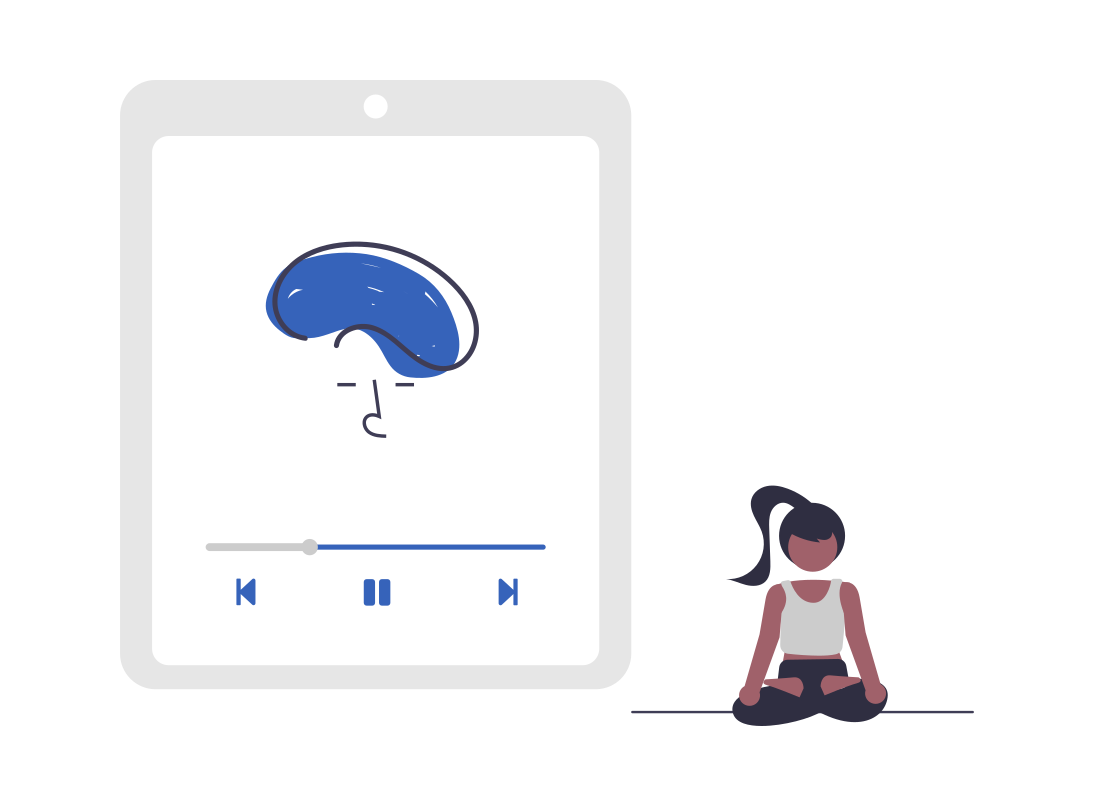
\includegraphics[height=0.35\textwidth]{./pics/undraw_Meditating_re_aiqa.png}
    \caption{Musik dient zur Entspannung}
\end{figure}

